\section{Statistiche sufficienti}
\begin{frame}[allowframebreaks]{List of things}
\printbibliography[keyword={inference},heading=beamer]
%\printbibliography[keyword={\mybibcat},heading=beamer]
\listofkeywords
\end{frame}

\subsection{Funzione di Likelihood}\linkdest{likelihood}

\begin{frame}{Funzione di Likelihood}
\begin{block}{Funzione di likelihood}
\begin{columns}[T]
\begin{column}{0.5\textwidth}
\[L_{x_0}(m)=p(x_0;m)\]
x,y: eventi indipendenti:
\[L_{(x_0,y_0)}(m)=L_{x_0}(m)L_{y_0}(m)\]
\end{column}
\begin{column}{0.5\textwidth}
Definita a meno di costante moltiplicativa ($\log{L}$): invariante per cambiamento di osservabile (funzione solo dei dati)
\[L_{f(t_0)}(m)=|J(t_0)|L_{t_0}(m)\]
\end{column}
\end{columns}
\end{block}
\begin{columns}[T]
\begin{column}{0.5\textwidth}
\begin{block}{T di Bayes e likelihood}
Se posso definire una $p(\theta)$:
\begin{align*}
&p(\theta|x_0)=\frac{p(x_0|\theta)p(\theta)}{p(x_0)}\\
&\posterior{}=\frac{\likelihood{}\prior{}}{\int p(x_0|\theta)p(\theta)\,d\theta}
\end{align*}
\end{block}
\end{column}
\begin{column}{0.5\textwidth}
\begin{block}{Degree of belief}
Posterior ratio: $\frac{\Pi(\theta_1|x_0)}{\Pi(\theta_2|x_0)}=\frac{L_{x_0}(\theta_2)}{L_{x_0}(\theta_1)}\frac{\Pi(\theta_2)}{\Pi(\theta_1)}$.
\end{block}
\end{column}
\end{columns}
\begin{block}{Metodo di massima likelihood}
Ripetendo gli esperimenti la likelihood diventa pi\'u piccata.
\end{block}
\end{frame}

\begin{frame}{Esempi di Likelihood: uniforme, bernoulli, ...}
\begin{block}{\mykeyword{Likelihood per distro uniforme}}
\pgfmathsetmacro{\unifM}{3}
\begin{columns}[T]
\begin{column}{0.5\textwidth}
\begin{tikzpicture}[scale=0.5,domain=0:1.5*\unifM]
\pgfmathsetmacro{\unifN}{(\unifM)^-1}
\begin{axis}[ylabel={$p(x;m)$},extra x ticks={\unifM}, extra x tick labels={$m$},
        extra x tick style={xticklabel style={yshift=-10}}]
%\draw[->] (-0.2,0) -- (1.5*\unifM,0) node[right] {$x$};
%\draw[->] (0,-0.2) -- (0,1.5*\unifM) node[above,red] {$p(x;m)$};
%\draw[color=red] plot[domain=0:\unifM, id=unif] function{\unifN} node[right] {$\frac{1}{m}$};
    \addplot[color=red] function [raw gnuplot, id=unifpdf, mark=none]{set xrange [0:\unifM]; plot \unifN};
\end{axis}
\end{tikzpicture}
\end{column}
\begin{column}{0.5\textwidth}
\begin{tikzpicture}[scale=0.5]
\begin{axis}[ylabel={$\mathcal{L}_{x_0}(m)$},extra x ticks={\data},extra x tick labels={$x_0$},
        extra x tick style={xticklabel style={yshift=-10}}]
\pgfmathsetmacro{\data}{(rand+1)/2*\unifM}
\pgfmathsetmacro{\unifN}{(\unifM)^-1}
    \addplot[color=orange] function [raw gnuplot, id=unifL, mark=none]{set xrange [\data:*]; plot 1/x};
\end{axis}
\end{tikzpicture}
\end{column}
\end{columns}
\end{block}
\begin{columns}[T]
\begin{column}{0.5\textwidth}
    \begin{block}{Likelihood per distro uniforme}
\begin{align*}
&L_0=1-p\\
&L_1=p
\end{align*}
\end{block}
\end{column}
\begin{column}{0.5\textwidth}
\begin{block}{Likelihood di pi\'u misure e statistiche}
\begin{align*}
&\prob{(t,\tau)}=\frac{1}{\tau}\exp{-\frac{t}{\tau}}\\
&L_{(t_1,\ldots,t_n)}(\tau)=\prod_i^n\frac{1}{\tau}\exp{-\frac{t_i}{\tau}}\\
&=\frac{1}{\tau^n}\exp{-\frac{\sum t_i}{\tau}}=\frac{1}{\tau^n}\exp{-\frac{n\overline{t}}{\tau}}
\end{align*}
\end{block}
\end{column}
\end{columns}
\end{frame}

\begin{frame}{Esercizi su Likelihood applicata}
\mykeyword{Ex: likelihood pdf exp; decadimento in volo particella.}
Distribuzione esponenziale in x: quale z?
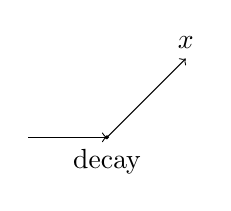
\begin{tikzpicture}
\draw[->] (0,0)--(1,0) node[draw,fill,circle,minimum size=1pt,inner sep=0,label=below:decay] {};
\draw[->] (1,0)--(2,1) node[above] {$x$};
\end{tikzpicture}
\end{frame}

\subsection{Statistiche sufficienti: teorema di fattorizzazione}\linkdest{statistiche}

\begin{frame}{Statistiche sufficienti per il parametro dato}
\begin{block}{Statistica sufficiente $S$ per parametro $\Theta$}
Pdf di X data $T(X)$ non dipende da parametro $\theta$:
 cio\'e pdf di $X$ dato $T(X)$ non dipende da $\theta$:
\[\prob{(x;S,\theta)}=\prob{(x;S)}\]
\end{block}
\begin{block}{Teorema di fattorizzazione}
Probabilit\'a di osservare $X$ dato $\theta$ \'e probabilit\'a di $T(x)$ dato $\theta$ per funzione sole osservabili: \[\prob{(x;\theta)}=\prob{(T(x);\theta)}h(x)\] e $\omega_{\theta}$ non dipende da $\theta$
\end{block}
\begin{block}{Statistica sufficiente minimale}
$S$ sufficiente e esiste una funzione $f$ per ogni $s_i$ con $S=f(s_i)$ e $\dim({S})\leq\dim{(X)}$.
\end{block}
\end{frame}

\begin{wordonframe}{Statistiche sufficienti: esempi.}
$\vec{x}=\{x_1,\ldots,x_n\}$: $T(\vec{x})$ sufficiente iff $L(\vec{x},\theta)=g(T,\theta)h(\vec{x})$ e dominio $\omega_{\theta}$ non dipende da $\theta$. Statistiche: media campionaria $\overline{x}=\frac{\sum x_i}{N}$, varianza campionaria, etc
\begin{align*}
%&L(x;\mu,\sigma)=\frac{1}{\sqrt{2\pi}\sigma}\exp{-\frac{1}{2}\frac{(x-\mu)^2}{\sigma^2}}\\
%&\overline{x}=\frac{\sum x_i}{N}:\ %L(\overline{x};\mu)=\prod_iL(x_i;\mu,\sigma)=(\frac{1}{\sqrt{2\pi}\sigma})^N\exp{-\frac{1}{2}\frac{\sum_i(x_i-\mu)^2}{\sigma^2}}
\end{align*}
\begin{block}{n RV iid con pdf bernoulli p}
$X_1,\ldots,X_n$: iid con pdf di Bernoulli, supporto pdf $\chi=\{0,1\}$, parametro p nell'intervallo $(0,1)$:
\begin{align*}
&T=\sum X_i\to\{0,\ldots,n\}&\intu{con pdf binomiale}
&\prob{(X_1=x_1\cap\ldots X_n=x_n|T=t)}=0, t\neq\sum x_i\\
&=\prob{(\cap_iX_i=x_i|T=t)}=\frac{\prob{((\cap_iX_i=x_i)\cap(T=t))}}{\prob{(T=t)}}=\frac{\prob{(\cap_iX_i=x_i)}}{\prob{(T=t)}}\intu{se $\sum x_i=t$:}
&A=\{\cap_iX_i=x_i\}\subseteq B=\{T=t\}
\end{align*}
e poich\'e le $X_i$ sono indipendenti si ha
\begin{align*}
&\frac{\prod\prob{(X_i=x_i)}}{\prob{(T=t)}}=\frac{p^{\sum x_i}(1-p)^{n-\sum x_i}}{\binom{n}{t}p^t(1-p)^{n-t}}
\end{align*}
\end{block}
\begin{block}{n RV iid Poisson$(\lambda)$}
$X_1,\ldots,X_n$: iid con pdf di Poisson con parametro ignoto $\lambda$:
\begin{align*}
&\prob{(X_1=x_1\cap\ldots X_n=x_n|T=t)}=\prob{(\cap_iX_i=x_i|T=t)}\\
&\frac{\prob{((\cap_iX_i=x_i)\cap(T=t))}}{\prob{(T=t)}}=\frac{\prob{(\cap_iX_i=x_i)}}{\prob{(T=t)}},\ t=\sum x_i\\
&=\frac{\prod_i[\frac{\exp{-\lambda}\lambda^{x_i}}{x_i!}]}{\frac{\exp{-\lambda}(n\lambda)^t}{t!}}=\frac{t!}{\prod x_i!}n^{-t}
\end{align*}
\end{block}
\begin{block}{Gaussiana: media ignota, varianza nota}
\begin{align*}
&L(\overline{x};\mu)=\prod_iL(x_i;\mu,\sigma)=(\frac{1}{\sqrt{2\pi}\sigma})^N\underbrace{\exp{-\frac{N}{2}\frac{\sum_i(\overline{x}-\mu)^2}{\sigma^2}}}_{g(T,\theta)}\underbrace{\exp{-\frac{N}{2}\frac{\sum_i(x_i-\overline{x})^2}{\sigma^2}}}_{h(\vec{x})}
\end{align*}
La statistica ''media aritmetica'' \'e sufficiente per parametro $\mu$ della gaussiana (dominio gaussiana non dipende da $\mu$) (\mykeyword{Ex: pdf della media aritmetica})
\end{block}
\begin{block}{Gaussiana: media nota, varianza ignota}
$\hat{\sigma}^2=\frac{\sum x_i^2-\mu}{N}$ \'e sufficiente per $\sigma^2$ (pdf di $\hat{\sigma}^2\propto g$ e dominio gaussiana non dipende da $\sigma$). (\mykeyword{Ex: statistica sufficiente $\sigma$ gaussiana})
\end{block}
\begin{block}{\mykeyword{Media aritmetica \'e statistica sufficiente per parametro binomiale, poissoniana, esponenziale }}
\begin{align*}
&\prob{(k)}=\binom{n}{k}p^k(1-p)^{n-k}\\
&\prob{(k)}=\frac{\mu^k\exp{-\mu}}{k!}\\
&\prob{(x)}=\lambda\exp{-\lambda x}
\end{align*}
\end{block}
\begin{block}{Distribuzione uniforme: \mykeyword{statistica $x_{max}$}.}
\begin{columns}[T]
\begin{column}{0.5\textwidth}
\pgfmathsetmacro{\unifM}{3}
\begin{tikzpicture}[scale=0.5,domain=0:1.5*\unifM]
\pgfmathsetmacro{\unifN}{(\unifM)^-1}
\begin{axis}[ylabel={$p(x;m)$},extra x ticks={\unifM}, extra x tick labels={$m$},
        extra x tick style={xticklabel style={yshift=-10}}]
%\draw[->] (-0.2,0) -- (1.5*\unifM,0) node[right] {$x$};
%\draw[->] (0,-0.2) -- (0,1.5*\unifM) node[above,red] {$p(x;m)$};
%\draw[color=red] plot[domain=0:\unifM, id=unif] function{\unifN} node[right] {$\frac{1}{m}$};
    \addplot[color=red] function [raw gnuplot, id=unifpdf, mark=none]{set xrange [0:\unifM]; plot \unifN};
\end{axis}
\end{tikzpicture}

\end{column}
\begin{column}{0.5\textwidth}
\begin{align*}
&\prob{(x;m)}=\left\{\begin{matrix}\frac{1}{m}\ x\in[0,m]\\0\\\end{matrix}\right.&\intertext{estraggo N $x_1,\ldots,x_n$}\\
&L(\vec{x},m)=\prod_iL(x_i;m)=\left\{\begin{matrix}\frac{1}{m^N}\ m>x_{max}\\0\ m<x_{max}\\\end{matrix}\right.
\end{align*}
\end{column}
\end{columns}
%$g(T,\theta)\propto A(T;\theta)$ dove $A$ \'e pdf di statistica $T$?
\begin{align*}
&\prob{(x_{max}<x_0)}=F_M(x_0)=\prod_i\prob{(x_i<x_0)}=\prod_i\int_0^{x_0}\frac{1}{m}\,dx=(\frac{x_0}{m})^N\\
&\prob{(x_M;m)}=\TDof{x_0}\left.F_M(x_0)\right|_{x_M}=\frac{N}{m}(\frac{x_M}{m})^{N-1}I(x_M<m)\\
&L_{\vec{x}}(m)=\frac{N}{m^N}x_M^{N-1}\frac{1}{Nx_M^{N-1}}=\prob{(x_M;m)}\frac{1}{Nx_M^{N-1}}\ m>x_M
\end{align*}
\end{block}
\mykeyword{Ex: distribuzione uniforme e statistica ''minimo campionario''}: Per pdf uniforme $x_{min}$ \'e sufficiente per m?
\end{wordonframe}

\subsection{Statistiche sufficienti: T di Darmois}

\begin{frame}{Teorema di Darmois}
\begin{block}{Teorema di Darmois: condizione necessaria e sufficiente per esistenza statistica sufficiente}
Esiste S tale che $\dim{(S)}<\dim{(X)}$ iff
\begin{align*}
&p(\vec{x}|\theta)=\Exp{[\sum_i^n\alpha_i(\vec{x})a_i(\theta)+\beta(\vec{x})+\gamma(\theta)}\ \text{\mykeyword{famiglia esponenziale}}\\
&S_j=\sum_i\alpha_j(x_i)
\end{align*}
\end{block}
Esiste statistica suff. iff: supporto pdf non dipende da parametro e appartiene alla famiglia esponenziale. In tal caso si ha:
\begin{align*}
&f(x;\theta)=\Exp{\alpha(x)a(\theta)+\beta(x)+c(\theta)}\\
&T=\sum_i\alpha(x_i)
\end{align*}
\end{frame}

\begin{wordonframe}{Famiglia esponenziale. Applicazioni del teorema di Darmois}
\begin{block}{Poisson}
\begin{align*}
&\frac{\exp{-\mu}\mu^k}{k!}=\exp{\mu}\exp{k\ln{\mu}}\exp{-\ln{k!}}\\
&S=\sum_i^Nk_i
\end{align*}
\end{block}
\begin{block}{Gaussiana: media ignota, varianza nota}
\begin{align*}
&L(\overline{x};\mu)=\prod_iL(x_i;\mu,\sigma)=(\frac{1}{\sqrt{2\pi}\sigma})^N\underbrace{\exp{-\frac{N}{2}\frac{\sum_i(\overline{x}-\mu)^2}{\sigma^2}}}_{g(T,\theta)}\underbrace{\exp{-\frac{N}{2}\frac{\sum_i(x_i-\overline{x})^2}{\sigma^2}}}_{h(\vec{x})}\\
&\alpha(x)=x\ \Rightarrow\ T=\frac{1}{N}\sum x_i=\exv{X}\\
&a(\mu)=\frac{\mu}{\sigma^2}\\
&\beta(x)=-\frac{x^2}{2\sigma}\\
&c(\mu)=
\end{align*}
La statistica ''media aritmetica'' \'e sufficiente per parametro $\mu$ della gaussiana (dominio gaussiana non dipende da $\mu$) (\mykeyword{Ex: pdf della media aritmetica})
\end{block}
\begin{block}{Gaussiana: media nota, varianza ignota}
$\hat{\sigma}^2=\frac{\sum x_i^2-\mu}{N}$ \'e sufficiente per $\sigma^2$ (pdf di $\hat{\sigma}^2\propto g$ e dominio gaussiana non dipende da $\sigma$). (\mykeyword{Ex: statistica sufficiente $\sigma$ gaussiana})
\begin{align*}
&L(\overline{x};\mu)=\prod_iL(x_i;\mu,\sigma)=(\frac{1}{\sqrt{2\pi}\sigma})^N\underbrace{\exp{-\frac{N}{2}\frac{\sum_i(\overline{x}-\mu)^2}{\sigma^2}}}_{g(T,\theta)}\underbrace{\exp{-\frac{N}{2}\frac{\sum_i(x_i-\overline{x})^2}{\sigma^2}}}_{h(\vec{x})}\\
&\alpha(x)=x\mu-\frac{x^2}{2}:\ T=\sum(x_i\mu-\frac{x_i^2}{2})\\
&a(\sigma^2)=\frac{1}{\sigma^2}\\
&\beta(x)=0\ c(\sigma^2)=-\frac{\mu^2}{2\sigma^2}-\ln{(\ldots)}\\
&\hat{\sigma}^2=\frac{\sum(x_i-\mu)^2}{N}=\frac{N\mu^2-2T}{N}
\end{align*}
\end{block}
\begin{block}{Applicazione allo spazio dei parametri completo della gaussiana}
\begin{align*}
&\log{\prob{(\vec{x};\mu,\sigma^2)}}=-\log{(\sqrt{2\pi}\sigma)}-\frac{x^2}{2\sigma^2}+\frac{x\mu}{2\sigma^2}+\frac{\mu^2}{2\sigma^2}\\
&\alpha_1(x)=x,\ a_1(\mu)=\mu,\ c=-\frac{\mu}{2\sigma^2}-\ln{(\sqrt{2\pi}\sigma)}\\
&\alpha_2(x)=-\frac{x^2}{2},\ a_2(\sigma^2)=\frac{1}{\sigma^2}\\
&S_{\mu}=\sum x_i,\ S_{\sigma^2}=-\sum\frac{x_i^2}{2}
\end{align*}
\end{block}
\mykeyword{Quale relazione tra numero statistiche sufficienti e parametri?}
\framebreak

\begin{block}{Media aritmetica \'e statistica sufficiente per parametro binomiale, poissoniana, esponenziale.}
\begin{columns}[T]
\begin{column}{0.33\textwidth}
\begin{align*}
&\prob{(k)}=\binom{n}{k}p^k(1-p)^{n-k}\intd{argomento di exp}
&\log{\binom{n}{k}}+k\log{\frac{p}{1-p}}\\
&+n\log{(1-p)}\\
&(\alpha(k)a(p)+\beta(k)+c(p))\\
&S=\sum_ik_i
\end{align*}
\end{column}
\begin{column}{0.33\textwidth}
\begin{align*}
&\prob{(k)}=\frac{\mu^k\exp{-\mu}}{k!}\intd{argomento di exp}
&k\log{\mu}-\mu-\log{k!}\\
&(\alpha(k)a(\mu)+\beta(k)+c(\mu))\\
&S=\sum_ik_i
\end{align*}
\end{column}
\begin{column}{0.33\textwidth}
\begin{align*}
&\prob{(x)}=\lambda\exp{-\lambda x}\intd{argomento di exp}
&-\lambda x-\mu+\log{\lambda}\\
&(\alpha(x)a(\lambda)+\beta(x)\\
&+c(\lambda))\\
&S=\sum_ix_i
\end{align*}
\end{column}
\end{columns}

\end{block}
\mykeyword{Ex: pdf non della famiglia esponenziale}: Come procedo se pdf non esponenziale (LHC)?
e\end{wordonframe}

\section{Inferenza statistica. Paradigma frequentista e bayesiano.}

%\begin{frame}[allowframebreaks]{List of keywords}%%mykeyword problems
%\listofkeywords
%\end{frame}

%\begin{refsection}{}
\subsection{Principio di sufficienza}

\begin{frame}{Principio di sufficienza}
\begin{block}{Principio di sufficienza}
Sia $E$ un esperimento con spazio campionario definito da $X$ e $S(X)$ una statistica sufficiente; sia $E'$ l'\mykeyword{esperimento derivato} con stesso spazio spazio dei parametri e tale che quando in $E$ \'e osservato x in $E'$ \'e osservato $t=t(x)$.
Principio di sufficienza: per ogni x $Ev(E,x)=Ev(E',t)$.
\end{block}
\begin{block}{Principio di likelihood (Fisher Barnard)}
    Se osservo x tutta informazione statistica in $L_x$: $L_x=L_y$ allora stesse inferenze da x e y. (Se $E$ e $E'$ hanno stesso spazio dei parametri e $x$, $y$ sono due misure le cui likelihood soddisfano $f(x,\theta)=cg(y,\theta)$ per ogni $\theta$ allora $Ev(E,x)=Ev(E',y)$
\end{block}
\end{frame}

\subsection{Principio di condizionalit\'a}

\subsection{Paradigmi di inferenza}

\begin{frame}{Paradigmi}
\begin{block}{Fisher}

\end{block}
\begin{block}{Neyman Pearson}

\end{block}
\begin{block}{Bayesian}
Il teorema di Bayes \'e usato per aggiornare la probabilit\'a sulla base di nuove informazioni. 
\end{block}
\end{frame}

\subsection{Baysiano}

\section{Stimatori}\linkdest{stimatori}

\begin{frame}{Propriet\'a generali stiamatori}
\begin{itemize}
    \item Consistenza (LGN): $\prob{\hat{\theta}}\to\theta_0$
    \item Varianza $\var{\vec{X}}\to\frac{1}{N}$/Bias $b(\vec{x})$ non diminuisce all'aumentare delle misure; scuola soggettivista: bias non esiste.
    \item distribuzione semplice
\end{itemize}
\end{frame}

\begin{frame}{Riduzione del bias}
\begin{columns}[T]
\begin{column}{0.5\textwidth}
$\PDy{\theta}{b}=0$ banale: $\E{[S]}=\alpha\theta$ si pone $S'=\frac{S}{\alpha}$
\end{column}
\begin{column}{0.5\textwidth}
Esempio:
\begin{align*}
&\E{[x_{max}]}=\frac{N}{N+1}m\\
&b(x_M)=-\frac{1}{N+1}m\\
&\hat{m}=\frac{N+1}{N}x_M\\
&\var{[\hat{m}]}=(\frac{N+1}{N})^2\var{[x_M]}
\end{align*}
\end{column}
\end{columns}
\begin{columns}[T]
\begin{column}{0.5\textwidth}
\begin{align*}
&\E{[S(x)]}=\theta+b(\theta)\\
&\to\ S'(x)=S(x)-b(\hat{\theta})-\hat{b}(x)\\
&\E{[\hat{b}(x)]}=b(\hat{\theta})\\
&\var{[S']}=\var{[S]}+\var{[b]}
\end{align*}
\end{column}
\begin{column}{0.5\textwidth}
Metodo empirico
\begin{align*}
&S_N'(x)=2S_N(x)\\
&-\frac{1}{2}[S_{\frac{N}{2}}(x_1,\ldots,x_{\frac{N}{2}})+S_{\frac{N}{2}}(x_{\frac{N}{2}},\ldots,x_N)]
\end{align*}
Supponendo $b_N\propto\frac{1}{N}$
\begin{align*}
&\E{[S_N']}=2\E{[S_N]}-\frac{1}{2}[2\E{[S_N]}]\\
&=2\theta+\frac{2c}{N}-\frac{1}{2}[2(\theta-\frac{2c}{N})]=\theta_0+o(\frac{1}{N^2})
\end{align*}
\end{column}
\end{columns}

\end{frame}

\subsection{Stimatori puntuali}\linkdest{points}

\begin{frame}{Stimatori puntuali}
\begin{columns}[T]
\begin{column}{0.33\textwidth}
Statistica $\hat{\Theta}(X_1,\ldots,X_n)$ che fornisce stima di funzione dei parametri $\tau(\Theta)$.
\end{column}
\begin{column}{0.67\textwidth}
\begin{itemize}
\item \mykeyword{unbiased estimator}: $\E_{\Theta}[T]=\tau(\Theta)$
\item \mykeyword{estimator bias}: $B_{\Theta}(T)=\E_{\Theta}[T]-\tau(\Theta)$
\item \mykeyword{Estimator mean square error}: $\E{[(T-\tau(\Theta))^2]}=V_{\Theta}[T]+(\E{[T]}-\tau(\Theta))^2$
\item \mykeyword{Stimatori consistenti}: $\lim_{n\to\infty}T_n(X_1,\ldots,X_n)\overset{P}{=}\tau(\Theta)$
\end{itemize}
\end{column}
\end{columns}
\end{frame}

\begin{frame}{Best unbiased estimator}
\begin{block}{Disuguaglianza di Cramer-Rao (CRLB)}
$X_1,\ldots,X_n$ iid con pdf $f(x,\Theta)$: se supporto $\Omega_{\Theta}$ di $f(x,\Theta)$ non dipende da $\Theta$ e integrali in $dx$ sono invertibili con $\PDof{\Theta}$; esiste stimatore unbiased $T(\vec{X})\xrightarrow{\E{[\ ]}}\tau(\Theta)$ con $\PDy{\Theta}{\tau}$ esiste finito, allora:
\begin{align*}
&V_{\Theta}[T]\geq\frac{[\tau'(\Theta)]^2}{n\E_{\Theta}[(\PDof{\Theta}\log{f(X_1;\Theta)})^2]}=\frac{[\tau'(\Theta)]^2}{nI_{X_1}(\Theta)}\\
&\left(\frac{(1+\TDy{\theta}{b})^2}{I_{\hat{\Theta}}(\theta)}\right)\intu{=: \mykeyword{minimum variance bound}}
\end{align*}
\end{block}
\begin{block}{Best unbiased estimator}
Uniformly minimum variance unbiased estimator such that $V_{\Theta}[T]\leq V_{\Theta}[T*]$ for all estimator $T^*$ unbiased.
\end{block}
\end{frame}

\begin{wordonframe}{Esempi di stimatori}
\begin{block}{Notazione}
$\Exp{X}=\frac{S_N}{N}$. Lo stimatore \'e un RV, la stima \'e un numero determinato sulla base della misura concreta.
\end{block}
\begin{block}{Stimatore per $\sigma^2$ di n iid gaussiane}
$X_1,\ldots,X_n$ n RV iid con pdf $N(\mu,\sigma^2)$. La varianza campionaria definita come $S^2=\frac{1}{n-1}\sum_i^n(x_i-\exv{X})^2$ \'e stimatore unbiased di $T(\Theta)=\sigma^2$
\end{block}
\begin{block}{Stimatore per $\mu$ di n iid gaussiane: CRLB per $\sigma$ noto}
$X_1,\ldots,X_n$ n RV iid con pdf $N(\mu,\sigma^2)$. $\exv{X}\to T(\mu)=\mu$; dato che $I_{X_1}=\sigma\expy{-2}$ la media campionaria \'e CRLB $\frac{\sigma^2}{n}=V_{\mu}[\exv{X}]$.
\end{block}
\begin{block}{Stimatore per $\lambda$ di n iid poissoniane}
$X_1,\ldots,X_n$ n RV iid con pdf $P(\lambda)$. $\exv{X}$ \'e stimatore di $T(\lambda)=\lambda$, $V_{\lambda}[\exv{X}]=\frac{\lambda}{n}$ quindi si raggiunge CRLB $\frac{\lambda}{n}$ ($I_{X_1}(\lambda)=\invers{\lambda}$).
\end{block}
\begin{block}{Stimatore per $p$ di n iid Bernoulli}
$X_1,\ldots,X_n$ n RV iiir has received mainly positive reviews. d con pdf $B(p)$. $\exv{X}$ \'e unbiased estimator of $\tau(p)=p$; dato che $I_{X_1}(p)=\frac{1}{p(1-p)}$, con $X_p[\exv{X}]=\frac{p(1-p)}{n}$ siamo al CRLB $\frac{p(1-p)}{n}$.
\end{block}
\begin{block}{Stimatori upper limit pdf uniforme: media aritmetica vs $x_{max}$.}
\begin{columns}[T]
\begin{column}{0.4\textwidth}
\begin{align*}
&\hat{m}_1=\frac{S_N}{N}=2\exv{X}\\
&b=\E{[\hat{m}_1]}-m=0\\
&\var{[\hat{m}_1]}=\frac{4Nm^2}{12N^2}
\end{align*}
\end{column}
\begin{column}{0.6\textwidth}
\begin{align*}
&p(x_{max};m)=\frac{N}{m^N}x_m^{N-1}\\
&\E{[x_{max}]}=\int_0^m\frac{N}{m^N}x_m^N\,dx_m=\frac{N}{N+1}\frac{m^{N+1}}{m^N}\intu{asintoticamente unbiased}
&\E{[x_{max}^2]}=\frac{N}{N+2}m^2-\frac{N^2}{(N+1)^2}m^2\\
&\var{[x_m]}=\E{[x_m^2]}-\E^2{[x_m]}\to0\\
&b(x_m)=-\frac{1}{N+1}m
\end{align*}
\end{column}
\end{columns}
\end{block}
\end{wordonframe}

\subsection{Informazione}\linkdest{informazione}

\begin{frame}{Informazione di Fischer}
Informazione contenuta nei dati su un parametro $\Theta$
\begin{align*}
&\overbrace{I_X(\Theta)}^{\text{n RV iid:}=nI_{X_1}}=\E_{\Theta}{[(\PDof{\Theta}\log{f(X;\Theta}))^2]}=\overbrace{-\E_{\Theta}{[\PtwoDof{\Theta}\log{f(X;\Theta)}]}}^{\text{se esistono finiti $\PtwoDof{\Theta}$ e $\E{}$}}
\end{align*}
Per due parametri:
\begin{align*}
&I_X(\Theta)=\begin{pmatrix}I_{11}(\Theta)&I_{12}(\Theta)\\I_{21}(\Theta)&I_{22}(\Theta)\end{pmatrix}\ I_{ij}(\Theta)=-\E{[\frac{\partial^2}{\partial\Theta_i\partial\Theta_j}\log{f(X;\Theta)}]}
\end{align*}
\begin{block}{Informazione e statistiche}
$I_X(\Theta)\geq I_T(\Theta)$: l'uguaglianza vale iff T \'e sufficiente per $\Theta$.
\end{block}
\begin{align*}
&Y=h(X)\ 1-1 \Rightarrow I_X=I_Y\\
&X\to f(X;\Theta)\ Y\to g(Y;\Theta)=f(\invers{h}(Y);\Theta)|\TDy{y}{\invers{h}(Y)}|\\
&I_Y=\E_Y{[(\PDof{\Theta}\log{g(Y)})^2]}=\E_Y{[(\PDof{\Theta}\log{f(\invers{h}(Y)})^2]}\\
&=\E_X{[(\PDof{\Theta}\log{f(X)})^2]}
\end{align*}
\end{frame}

\begin{wordonframe}{Esempi Informazione}
\begin{columns}[T]
\begin{column}{0.5\textwidth}
\begin{block}{pdf Poisson}
\begin{align*}
&\log{f}=-\lambda+x\log{\lambda}-\log{x!}\\
&I_X(\lambda)=\invers{\lambda}
\end{align*}
\end{block}
\end{column}
\begin{column}{0.5\textwidth}
\begin{block}{pdf Gauss}
\begin{align*}
&\log{f}=-\frac{1}{2}\frac{(x-\mu)^2}{\sigma^2}-\log{(\sqrt{2\pi}\sigma)}\\
&I_X(\mu)=\sigma\expy{-2}
\end{align*}
\end{block}
\end{column}
\end{columns}
\begin{block}{n RV iid}
\begin{columns}[T]
\begin{column}{0.5\textwidth}
$X_1,\ldots,X_n$ n RV iid:
\begin{align*}
&X=\sum X_i\\
&I_X(\Theta)=nI_{X_1}(\Theta)
\end{align*}
\end{column}
\begin{column}{0.5\textwidth}
proof pg 327 probability and statistical inference
\end{column}
\end{columns}
\end{block}
\begin{block}{n RV gaussiane $N(\mu,\sigma^2)$: matrice informazione}
$\vec{X}=(X_1,\ldots,X_n)$ e $\vec{\Theta}=(\mu,\sigma^2)$
\begin{align*}
&I_{11}=\E{[(\PDof{\mu}\log{f})^2]}=\sigma\expy{-2}\ I_{22}=\E{[(\PDof{\sigma^2}\log{f})^2]}=\frac{1}{2}\sigma\expy{-4}\\
&I_{12}=I_{21}=\frac{1}{2\sigma^2}\E{[\sigma\expy{-3}(X_1-\mu)^3-(X_1-\mu)]}=0
\end{align*}
\end{block}
\begin{block}{Perdita di informazione se tengo solo media campionaria delle RV gaussiane}
$\vec{X}=(X_1,\ldots,X_n)$ e media $\exv{X}=\frac{1}{n}\sum X_i$ con pdf $N(\mu,\invers{n}\sigma^2)=g(x,\Theta)=\frac{\sqrt{n}}{\sigma\sqrt{2\pi}}\exp{-\frac{n}{2\sigma^2}(x-\mu)^2}$
\begin{align*}
&I_{11}=\E{[(\PDof{\mu}\log{g})^2]}=n\sigma\expy{-2}\ I_{22}=\E{[(\PDof{\sigma^2}\log{g})^2]}=\frac{1}{2}\sigma\expy{-4}\\
&I_{12}=I_{21}=\frac{1}{2\sigma^2}\E{[\sigma\expy{-3}(X_1-\mu)^3-(X_1-\mu)]}=0\\
&I_{\vec{X}}-I_{\exv{X}}\geq0
\end{align*}
\end{block}
\begin{block}{Perdita di informazione se tengo solo la varianza campionaria delle RV gaussiane}
Varianza campionaria $S^2=\frac{1}{n-1}\sum_i(X_i-\exv{X})^2$ (\mykeyword{Gaussian variance: unbiased estimator}). 
La RV $Y=(n-1)\frac{S^2}{\sigma^2}$ ha pdf $\chi^2_{n-1}$: $c\exp{-\frac{1}{2}y}y\expy{\frac{n-3}{2}}$ con $c=2\expy{\frac{n-1}{2}}\Gamma(\frac{1}{2}(n-1))$
\begin{align*}
&S^2\to h(x;\theta)=d\sigma\expy{-(n-1)}\exp{-\frac{n-1}{2}\frac{x}{\sigma^2}}x\expy{\frac{n-3}{2}}\ d=c(n-1)^{\frac{n-1}{2}}\\
&I_{11}=I_{12}=I_{21}=0\ I_{22}=\frac{1}{2}(n-1)\sigma\expy{-4}:\\ &I_{\vec{x}}-I_{S^2}=\begin{pmatrix}n\sigma\expy{-2}&0\\0&\frac{1}{2}\sigma\expy{-4}\end{pmatrix}''\geq0''
\end{align*}
$\exv{X}$, $S^2$ are indipendently ($P(A\cap B)=P(A)P(B))$) distributed: $I_{\exv{X},S^2}=I_{\exv{X}}+I_{S^2}=I_{\vec{X}}(\Theta)$.
\end{block}
\begin{block}{Poissoniana}
$k_1,\ldots,k_n$ n RV iid poissoniane $f(k,\mu)=\frac{\mu^k\exp{-\mu}}{k!}$:
\begin{align*}
&I_k(\mu)=-\E{[\PtwoDy{\mu}{\log{(L)}}]}=N(-\E{[\PtwoDy{\mu}{\log{(p(k;\mu))}}]})\\
&\PtwoDy{\mu}{\log{(p(k;\mu)}}=-\frac{k}{\mu^2}\\
&I_k(\mu)=N\E{[\frac{k}{\mu}]}=\frac{N}{\mu}\\
&S=\sum k_i,\ f(S;\mu)=\frac{(N\mu)^S\exp{-N\mu}}{S!},\ I_s(\mu)=\frac{N}{\mu}
\end{align*}
$I_s=I_k$ poich\'e $S$ \'e statistica sufficiente.
\end{block}
\begin{block}{Binomiale}
\begin{align*}
&I_k(p)=-N\E{[\PtwoDy{p}{\log{f(k;n,p)}}]}=N\frac{n}{p(1-p)}\\
&S=\sum_ik_i:\ f(S;nN,p)=\binom{nN}{S}p^S(1-p)^{nN-S}
\end{align*}
\mykeyword{Ex: Informazione di binomiale e statistica suff.}
\end{block}
\begin{block}{Ex: Pdf uniforme e minimum variance bound per $x_M$}
\begin{align*}
&I_{X_1}=I_{x_m}(m)=\frac{N^2}{m}\\
&\var{[\hat{\theta},\theta]}=\frac{N}{(N+2)(N+1)^2}m\overset{??}{\geq}\frac{(1+\TDy{\theta}{b})^2}{I_{\hat{\theta}}(\theta)}=\frac{(1-\frac{1}{N+1})^2}{\frac{N^2}{m^2}}
\end{align*}
\mykeyword{Ex: Pdf uniforme e minimum variance bound per $x_m$}
\end{block}
\framebreak
\begin{block}{\mykeyword{Statistica $x_{min}$ per pdf uniforme}}
pdf di $x_{min}$
\begin{columns}[T]
\begin{column}{0.5\textwidth}
Trasformazione di variabile
\begin{align*}
&x'\to m-x\\
&f(x_m;m)=\frac{N}{m}[1-\frac{x_m}{m}]^{N-1}I(x\leq m)
\end{align*}
\end{column}
\begin{column}{0.5\textwidth}
\mykeyword{Ex: pdf $x_{min}$ (cumulanti)}
\begin{align*}
&F(x_0)=\prob{[x_m>x_0]}\\
&\prob{(\{x_i\}>x_0)}=[\int_{x_0}^m\frac{dx}{m}]^N\\
&=[1-\frac{x_0}{m}]^N
\end{align*}
\end{column}
\end{columns}
\end{block}
\begin{block}{Statistica $x_m$ non \'e consistente}
\begin{align*}
&\E{[x_m]}=\int\,dx_mx_mf(x_m;m)=\int\,dx_mx_m\frac{N}{m}[1-\frac{x_m}{m}]^{N-1}=\frac{m}{N+1}\\
&\E{[x_m^2]}=\int\,dx_mx_m^2f(x_m;m)=\int\,dx_mx_m^2\frac{N}{m}[1-\frac{x_m}{m}]^{N-1}\\
&=\frac{2m^2}{(N+1)(N+2)}\\
&\var{[x_m]}=\E{[x_m^2]}-\E^2{[x_m]}=\frac{N}{(N+1)^2(N+2)}m^2\to0\\
&\hat{m}=(N+1)x_m:\ \E{[\hat{m}]}=m,\ \var{[\hat{m}]}=\frac{N^2}{(N+1)(N+2)}m^2\\
&I_{x_m}(m)=\frac{N}{(N-2)m^2},\ (CR:\ \frac{N}{N+2}\geq\frac{N-2}{N})
\end{align*}
$\hat{m}$ non \'e consistente: non converge in probabilit\'a al parametro.
\end{block}
\end{wordonframe}

\begin{frame}{Come ridurre i dati se statistica sufficiente non \'e disponibili}
Perdita informazione
\begin{itemize}
\item istogramma
\item dati troncati
\end{itemize}
\end{frame}

\subsection{Metodi costruzione stimatori consistenti}\linkdest{methodsestimators}

\begin{frame}{Momenti}\frameintoc
\begin{columns}[T]
\begin{column}{0.6\textwidth}
\begin{block}{Momenti campionari: stimatori consistenti}
\begin{align*}
&m_k=\frac{\sum_ix_i^k}{N}\\
&\E{[m_k]}=\frac{\sum_i\E{[x_i^k]}}{N}=\mu'\intu{convergono in probabilit\'a ai momenti della distribuzione}
&\cov{(m_i,m_j)}=\E{[m_im_j]-\E{[m_i]}\E{[m_j]}}\\
&=\frac{\mu'_{i+j}-\mu_i'\mu_j'}{N}
\end{align*}
\end{block}
\end{column}
\begin{column}{0.5\textwidth}
\begin{align*}
&m_1=\mu_1'(\theta_1,\ldots,\theta_n)\\
&\vdots\\
&m_n=\mu_n'(\theta_1,\ldots,\theta_n)\intd{Invertendo il sistema sopra si trovano gli stimatori:}
&\hat{\theta_1}(m_1,\ldots,m_n)\\
&\vdots\\
&\hat{\theta_1}(m_1,\ldots,m_n)
\end{align*}
\end{column}
\end{columns}
\end{frame}

\begin{frame}{Stimatori impliciti}\frameintoc
\begin{align*}
&\E_{\theta}[g(X,\theta_0)]=0,\ \forall\theta:\ \int f(x;\theta_0)p(x;\theta)\,dx=0,\ h(\theta_0)=0\\
&(f(x,\theta)=S(x)-\E_{\theta}{[S]},\ \E{[f]}=\E_{\theta_0}{[S]}-\E_{\theta}{[S]})\\
&K_N(\vec{X},\theta)=\frac{1}{N}\sum_if(x_i,\theta)\intu{stimatore consistente di $h(\theta)$:}
&K_N(\vec{X},\theta)\to\E{[f(\vec{X},\theta)]}
\end{align*}
Se $K_N(x)$ \'e $C^1$ e $\lim_{N\to\infty}\left.\E{[\PDy{\theta}{K_N}]}\right|_{\theta_0}\neq0$: almeno una soluzione dell'equazione $K_N(\vec{X},\hat{\theta})=0$ \'e stimatore consistente.
\end{frame}

\begin{frame}{Massima likelihood}\frameintoc
\begin{block}{Derivazione metodo massima likelihood da stimatori impliciti. Score di Fisher}
\begin{align*}
&f(x,\theta)=\PDy{\theta}{\log{L}}:\ K_N=\frac{1}{N}\sum_i\PDy{\theta}{\log{(L(x_i,\theta))}}=0\\
&\E{[\left.\PDy{\theta}{\log{L}}\right|_{\theta_0=\hat{\theta}}]}=0\ (\hat{\theta}(\vec{x}):\ L(\hat{\theta})=\sup_{\theta}L(\theta))\intd{$\hat{\theta}$ \'e massimo per $L$ dato che}
&\E{[\PDy{\theta}{K}]}=\E{[\PtwoDy{\theta}{\log{L}}]}=-I_X<0
\end{align*}
\end{block}
\end{frame}

\begin{frame}[allowframebreaks]{Propriet\'a MLE}
\begin{block}{Consistente se soluzione della likelihood equation \'e unica: massimo assoluto (asintotico) \'e consistente}
$\PDy{\theta}{\log{L_{tot}}}=0$.
\end{block}
\begin{block}{Invariante per trasformazione di parametro}
\end{block}
\begin{block}{Asintoticamente un-biased}
\end{block}
\begin{block}{Asintoticamente efficente: $\var{[\hat{\theta}]}\to\frac{1}{NI_{X_1}}$}
\begin{align*}
&K_N(\hat{\theta)}=K(\theta_0)+\PDy{\theta}{K_N}(\hat{\theta}-\theta_0)+o(\hat{\theta}-\theta_0)^2\intd{prendendo il valore di aspettazione}
&0=\sum_i\frac{\PDy{\theta}{\log{(L(x_i))}}}{N}-I(\hat{\theta}-\theta_0)+(\var{[\hat{\theta}]})\\
&\hat{\theta}-\theta_0\propto N(0,\frac{1}{NI})+\frac{\const{}}{N}: \lim_{N\to\infty}b(\hat{\theta})\propto\frac{1}{N}
\end{align*}
\end{block}
\cite{barlow1990extended}
\end{frame}

\begin{wordonframe}{MLE in pratica}
\begin{block}{binning}
\begin{columns}[T]
\begin{column}{0.5\textwidth}
N fissato
\begin{align*}
&\prob{(\vec{k},\theta)}=\frac{N!}{\prod_ik_i!}\prod_i{\underbrace{\prob{(i)}}_{\int_{S_i}\prob{(x|\theta)}\,dx}}\mkern-20mu^{k_i}\\
&\max{[\sum_i k_i\log{[\prob{(x;\theta)}\Delta]}]}\\
&\to\max{[\sum_i \log{[\prob{(n_i;\theta)}]}]}
\end{align*}
\end{column}
\begin{column}{0.5\textwidth}
N variabile: \mykeyword{Extended likelihood}, normalizzazione varia
\begin{align*}
&\mu_i=\mu_TP_i(\theta)\\
&\prob{(k_i\theta)}=\frac{\prod_i\exp{-\mu_TP_i}(\mu_TP_i)^{k_i}}{k_i!}\\
&\log{L}=\sum_ik_i\log{P_i(\theta)}+k_i\log{\mu_T}\\
&-\mu_TP_i-\bcancel{\log{k!}}\\
&\left\{\begin{matrix}\mkern-240mu\PDy{\theta_i}{\log{L}}=0\\\PDy{\mu_T}{\log{L}}=0\ (:L(\bcancel{\mu_T}),\mu_T(\bcancel{\theta_i}) \Rightarrow\ \mu_T=N)\\\end{matrix}\right.
\end{align*}
\end{column}
\end{columns}
\end{block}
\begin{block}{Fit resolution of histogram (??)}
$A=\sum_i\frac{1}{P_i}(\PDy{\theta}{P_i})^2$
\end{block}\end{wordonframe}

\begin{frame}{Massima likelihood: metodo minimi quadrati}\frameintoc
Se i conteggi (binned case) sono distribuiti in maniera normale attorno al valore $\mu_TP_i$ la minimizzazione del $\chi^2$ \'e equivalente alla massimizzazione della likelihood
\begin{align*}
&\prob{(k_i,\theta)}\propto\exp{-\frac{(k_i-\mu_i)^2}{2\sigma_i^2}}\intd{$\log{L}$ \'e massimizzato dalla funzione che minimizza}
&\chi^2=-2\log{L}=\sum_i\frac{(k_i-\mu_i(\theta))^2}{\sigma_i^2}\intd{if measures are not indipendent}
&\log{(L(\theta))}=-\frac{1}{2}\sum_{ij}(y_i-\lambda_i(\theta))[\invers{V}]_{ij}(y_j-\lambda_j(\theta))
\end{align*}

(se $W_{ij}>0$: $\PDy{\theta}{\mu_i}W_{ij}\PDy{\theta}{\mu_j}\geq0$??)
\mykeyword{Estimators:Least square examples in cowan 95}
\end{frame}

\begin{frame}{Best linear unbiased estimator. Teorema di Gauss-Markov}
\begin{block}{Funzioni lineari dei parametri}
se $\lambda_i(\theta)=\mu_i(\theta)=\sum_ja_j(\vec{x})\theta_j$, $a_j(\vec{x})$ lin. indip., allora $\hat{\theta}_j$ sono unbiased e al MVB: teorema di Gauss-Markov.
Per dati da gaussiana multi-dimensionale con $\vec{\mu}$ ignota ma covarianza $V$ nota
\begin{align*}
&\chi^2=(\vec{y}-\vec{\lambda})^T\invers{V}(\vec{y}-\vec{\lambda})=(\vec{y}-A\vec{\theta})^T\invers{V}(\vec{y}-A\vec{\theta})\intd{e la condizione di minimo}
&\nabla\chi^2=-2(A^T\invers{V}\vec{y}-A^T\invers{V}A\vec{\theta})=0\intd{che ha soluzione}
&\hat{\vec{\theta}}=\invers{()}A^T\invers{V}\vec{y}=B\vec{y}\intd{e matrice di covarianza:}
&U=BVB^T=\invers{(A^TVA)}=\cov{(\theta_i,\theta_j)},\ [\invers{U}]_{ij}=\frac{1}{2}\left[\frac{\partial^2\chi^2}{\partial\theta_i\partial\theta_j}\right]|_{\theta=\hat{\theta}}
\end{align*}
\end{block}
\begin{block}{Contours in parameter space}
\begin{align*}
&\chi^2(\theta)=\chi^2(\hat{\theta})+\frac{1}{2}\sum_{ij}\left[\frac{\partial^2\chi^2}{\partial\theta_i\partial\theta_j}\right]|_{\theta=\hat{\theta}}(\theta_i-\hat{\theta}_i)(\theta_j-\hat{\theta}_j)
\end{align*}
contours in parameter space whose tangents are $\hat{\theta}_i\pm\hat{\sigma}_i$:
\begin{align*}
&\chi^2(\vec{\theta})=\chi^2(\hat{\theta})+1
\end{align*}
\end{block}
\end{frame}